\chapter{U-Sem plug-in environment tutorial} 
\label{cha:tutorial}

In this tutorial we demonstrate how to create and deploy U-Sem plug-ins. 

\section{Requirements}

\begin{itemize}
	\item U-Sem - installed and running
	\item Eclipse IDE ($>=$ 3.7 Indigo). We recommend using the \textit{Eclipse for RCP and RAP Developers} package - \url{http://www.eclipse.org/downloads/}
	\item U-Sem SDK for Eclipse - \url{https://code.google.com/p/rdfgears/}
\end{itemize}

\section{Set-up the IDE}

Before being able to start developing plug-ins for U-Sem we have to set up the IDE. This process consists of two main steps:

\subsection{Import the U-Sem core project}

Plug-ins normally depend on functionality provided by the U-Sem project and therefore, in order to be able to compile them correctly we need to import the U-Sem project into the IDE. Currently, all dependencies are contained in the \textbf{rdfgears-core} sub-project and thus, importing only it is enough. For more information on importing existing projects in eclipse read the \textit{Importing existing projects} section in Eclipse documentation(\url{http://help.eclipse.org/juno}).

\subsection{Install the U-Sem SDK}
U-Sem comes with SDK that helps engineers to easily create plug-ins. It provides project template which creates and automatically makes all necessary configurations for a plug-in project. In order to install it copy the SDK jar file to the \textit{dropins} folder of Eclipse and start/restart the IDE. 

\section{Create plug-in}

\subsection{Step 1 - Create plug-in project}
	In order to create new plug-in project for U-Sem the following steps has to be followed:
	\begin{enumerate}
		\item Open the \textit{New plug-in wizard} in Eclipse - it can be found under File/New/Plug-in Project
		\item Fill in all standard configuration details and click next until the \textit{Templates} section appears

\begin{figure}
  \centering
    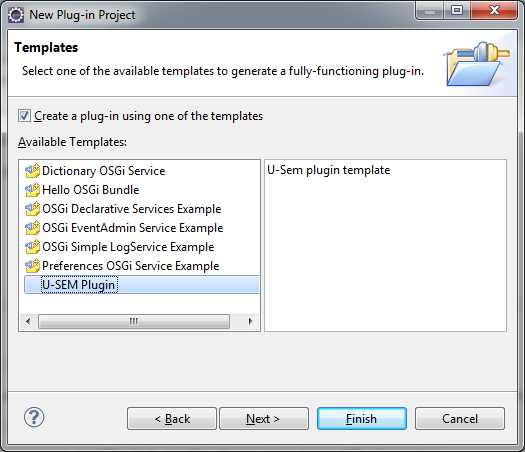
\includegraphics[width=0.8\textwidth]{apendix/PluginTutorial/wiz_templ.png}
    \caption{Select plug-in template}
    \label{templ}
\end{figure}

		\item Select the \textit{U-Sem} template and click next. The window is shown on Figure \ref{templ}.
		\item The plug-in template creates sample RDF Gears function and workflow which are wired to work together. Users have to specify their names. Figure \ref{art}
		
\begin{figure}
  \centering
    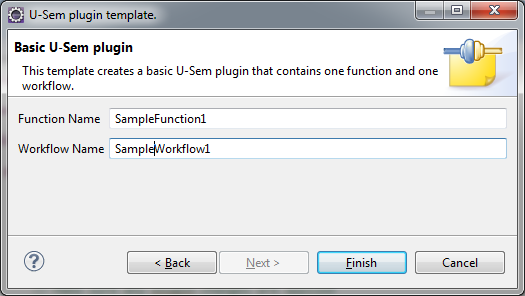
\includegraphics[width=0.6\textwidth]{apendix/PluginTutorial/wiz_art.png}
    \caption{Specify artefact names}
    \label{art}
\end{figure}

		\item Click Finish and the plug-in is automatically created and configured. The newly created project has the structure showed in Figure \ref{struct}
		
\begin{figure}
  \centering
    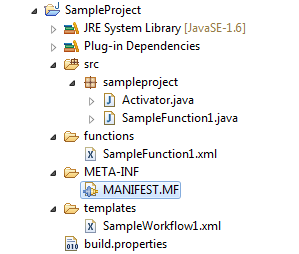
\includegraphics[width=0.5\textwidth]{apendix/PluginTutorial/fileStruct.png}
    \caption{Structure of the created plug-in}
    \label{struct}
\end{figure}

	\end{enumerate}

\subsection{Step 2 - Create U-Sem artefacts manually}
Engineers can also add U-Sem artefacts (functions, workflows) manually. In order to do that, the following steps has to be performed:

\begin{enumerate}
	\item \textbf{Create artefacts} - Engineers have to create the desired U-Sem functions and workflows following the specification(\url{https://code.google.com/p/rdfgears/wiki/Creating_cstom_functions}). The produced files has to be added to the plug-in project.
	\item \textbf{Register the artefacts} - The already produced artefacts has to be registered so that the engine knows about their existence. The registration is done in the \textit{start} method of the \textit{Activator} java class:
	\begin{itemize}
	
		\item In order to register functions the following code has to be included:
		
\begin{lstlisting}
context.registerService(FunctionDescriptor.class, 
  new FunctionDescriptor(getClass().getResourceAsStream("/<xml>"), 
  <class>), null)
\end{lstlisting}

		Where \textit{$<xml>$} is the path to the xml file describing the function and \textit{$<class>$} is the java class that contains function's logic.
		
		\item In order to register workflows the following code has to be included: 
\begin{lstlisting}
context.registerService(WorkflowTemplate.class,
  new WorkflowTemplate(getClass().getResourceAsStream("/<xml>")),
  null);
\end{lstlisting}

		Where \textit{$<xml>$} is the path to the xml file describing the workflow.
		
	\end{itemize}
	\item \textbf{Configure plug-in export} -  Before exporting the plug-in make sure all resource files (xml, etc.) will be included. More information on how to do that can be found under the \textit{Plug-in Build} section in Eclipse documentation(\url{http://help.eclipse.org/juno}).
	
	
\end{enumerate}

\subsection{Step 3 - Export the project}
Once the plug-in is ready then it has to be exported into a jar file so that it can be later deployed to the U-Sem platform. Eclipse provides wizard that completely automates this process. It is accessible under \textit{File/Export/Deployable plug-ins and fragments}. More information about it can be found under the \textit{Plug-in Export} section in Eclipse documentation(\url{http://help.eclipse.org/juno}).

\section{Install plug-ins in U-Sem}

\begin{figure}
  \centering
    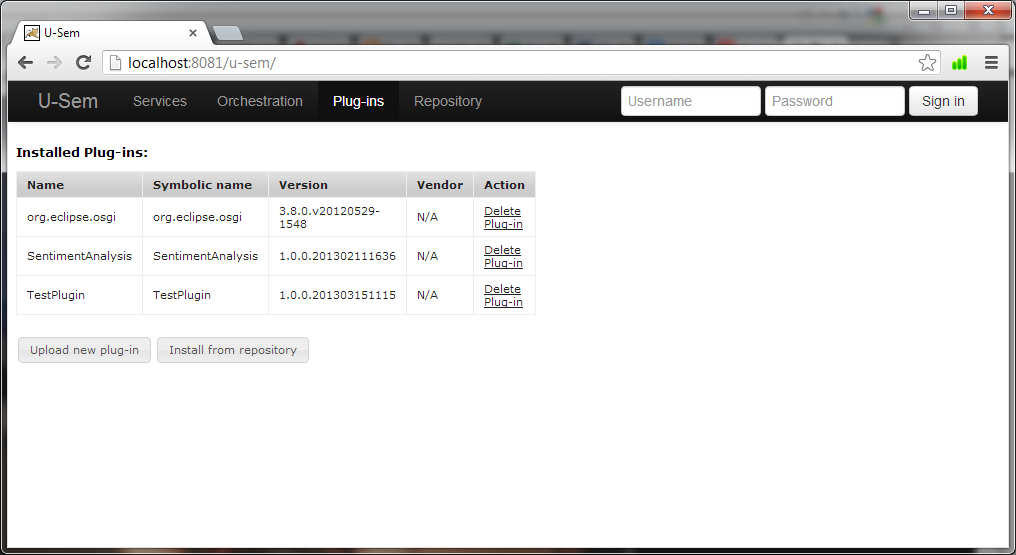
\includegraphics[width=0.8\textwidth]{apendix/PluginTutorial/plugin-list.png}
    \caption{U-Sem Plug-ins user interface}
    \label{plugin-list}
\end{figure}

The functionality for installing a plug-in to the U-Sem platform is available under the \textit{Plug-ins} section in the user interface of U-Sem shown on Figure \ref{plugin-list}. Users have to click on the \textit{Upload new plug-in} button which will enable them to select a plug-in to be installed. This is shown on Figure \ref{plugin-upload}. Finally, after the successful installation of the plug-in all artefacts provided by it will be available to use in U-Sem. 

\begin{figure}
  \centering
    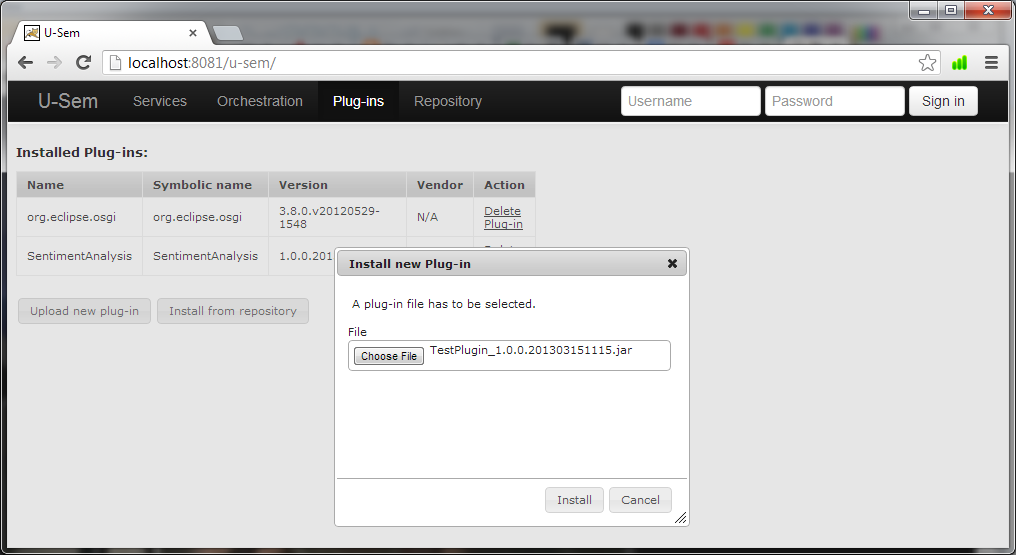
\includegraphics[width=0.8\textwidth]{apendix/PluginTutorial/plugin-upload.png}
    \caption{UI for selecting a plug-in to be installed}
    \label{plugin-upload}
\end{figure}
